\documentclass{article}

\usepackage{tikz}
\usetikzlibrary{shapes,arrows}

\begin{document}

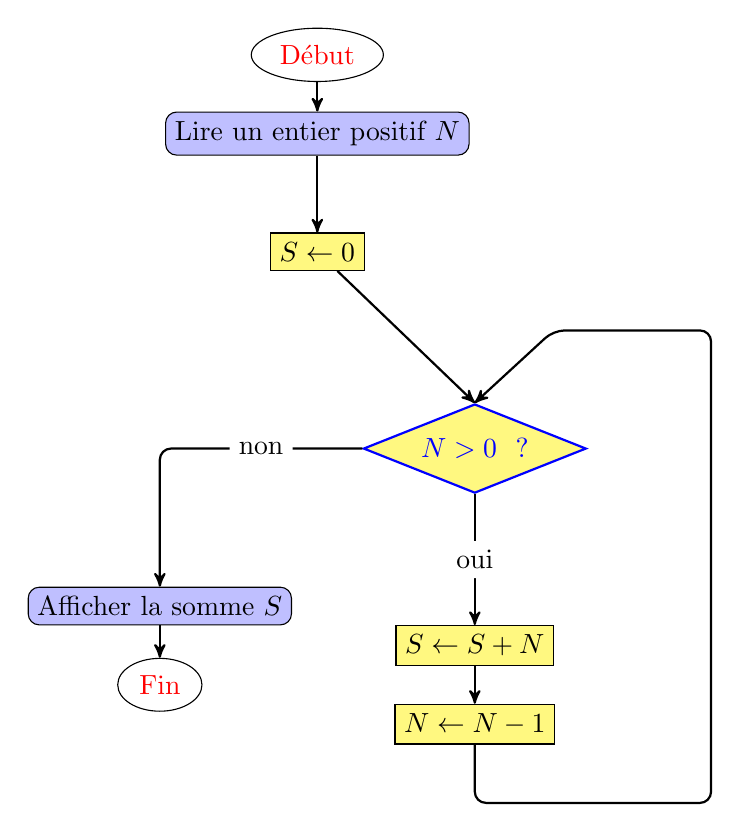
\begin{tikzpicture}
 % style des noeuds
  \tikzstyle{debutfin}=[ellipse,draw,text=red]
  \tikzstyle{instruct}=[rectangle,draw,fill=yellow!50]
  \tikzstyle{test}=[diamond, aspect=2.5,thick,thick,draw=blue,fill=yellow!50,text=blue]
  \tikzstyle{es}=[rectangle,draw,rounded corners=4pt,fill=blue!25]
 % style des fleches
  \tikzstyle{suite}=[->,>=stealth',thick,rounded corners=4pt]
 % placement des noeuds
  \node[debutfin] (debut) at (-2,5) {D\'ebut};
  \node[es] (lire) at (-2,4) {Lire un entier positif $N$};
  \node[test] (test) at (0,0) {$N>0$ \  ?};
  \node[instruct] (init) at (-2,2.5) {$S\leftarrow 0$};
  \node[instruct] (plus) at (0,-2.5) {$S\leftarrow S+N$};
  \node[instruct] (moins) at (0,-3.5) {$N\leftarrow N-1$};
  \node[es] (afficher) at (-4,-2) {Afficher la somme $S$};
  \node[debutfin] (fin) at (-4,-3) {Fin};
 % Placement des fleches
  \draw[suite] (debut) -- (lire);
  \draw[suite] (lire) -- (init);
  \draw[suite] (init) -- (test.north);
  \draw[suite] (test) -- (plus) node[midway,fill=white]{oui};
  \draw[suite] (plus) -- (moins);
  \draw[suite] (moins) |- (3,-4.5) |- (1,1.5) -- (test.north);
  \draw[suite] (test) -| (afficher) node[near start,fill=white]{non};
  \draw[suite] (afficher) -- (fin);
\end{tikzpicture}

\end{document}
